\documentclass[tikz,border=12pt]{standalone}
\usepackage{tikz}
\usepackage{amsmath,amssymb}
\usepackage{helvet}
\renewcommand{\familydefault}{\sfdefault}
\usetikzlibrary{positioning, arrows.meta, shapes.geometric, fit, backgrounds, calc}

\begin{document}
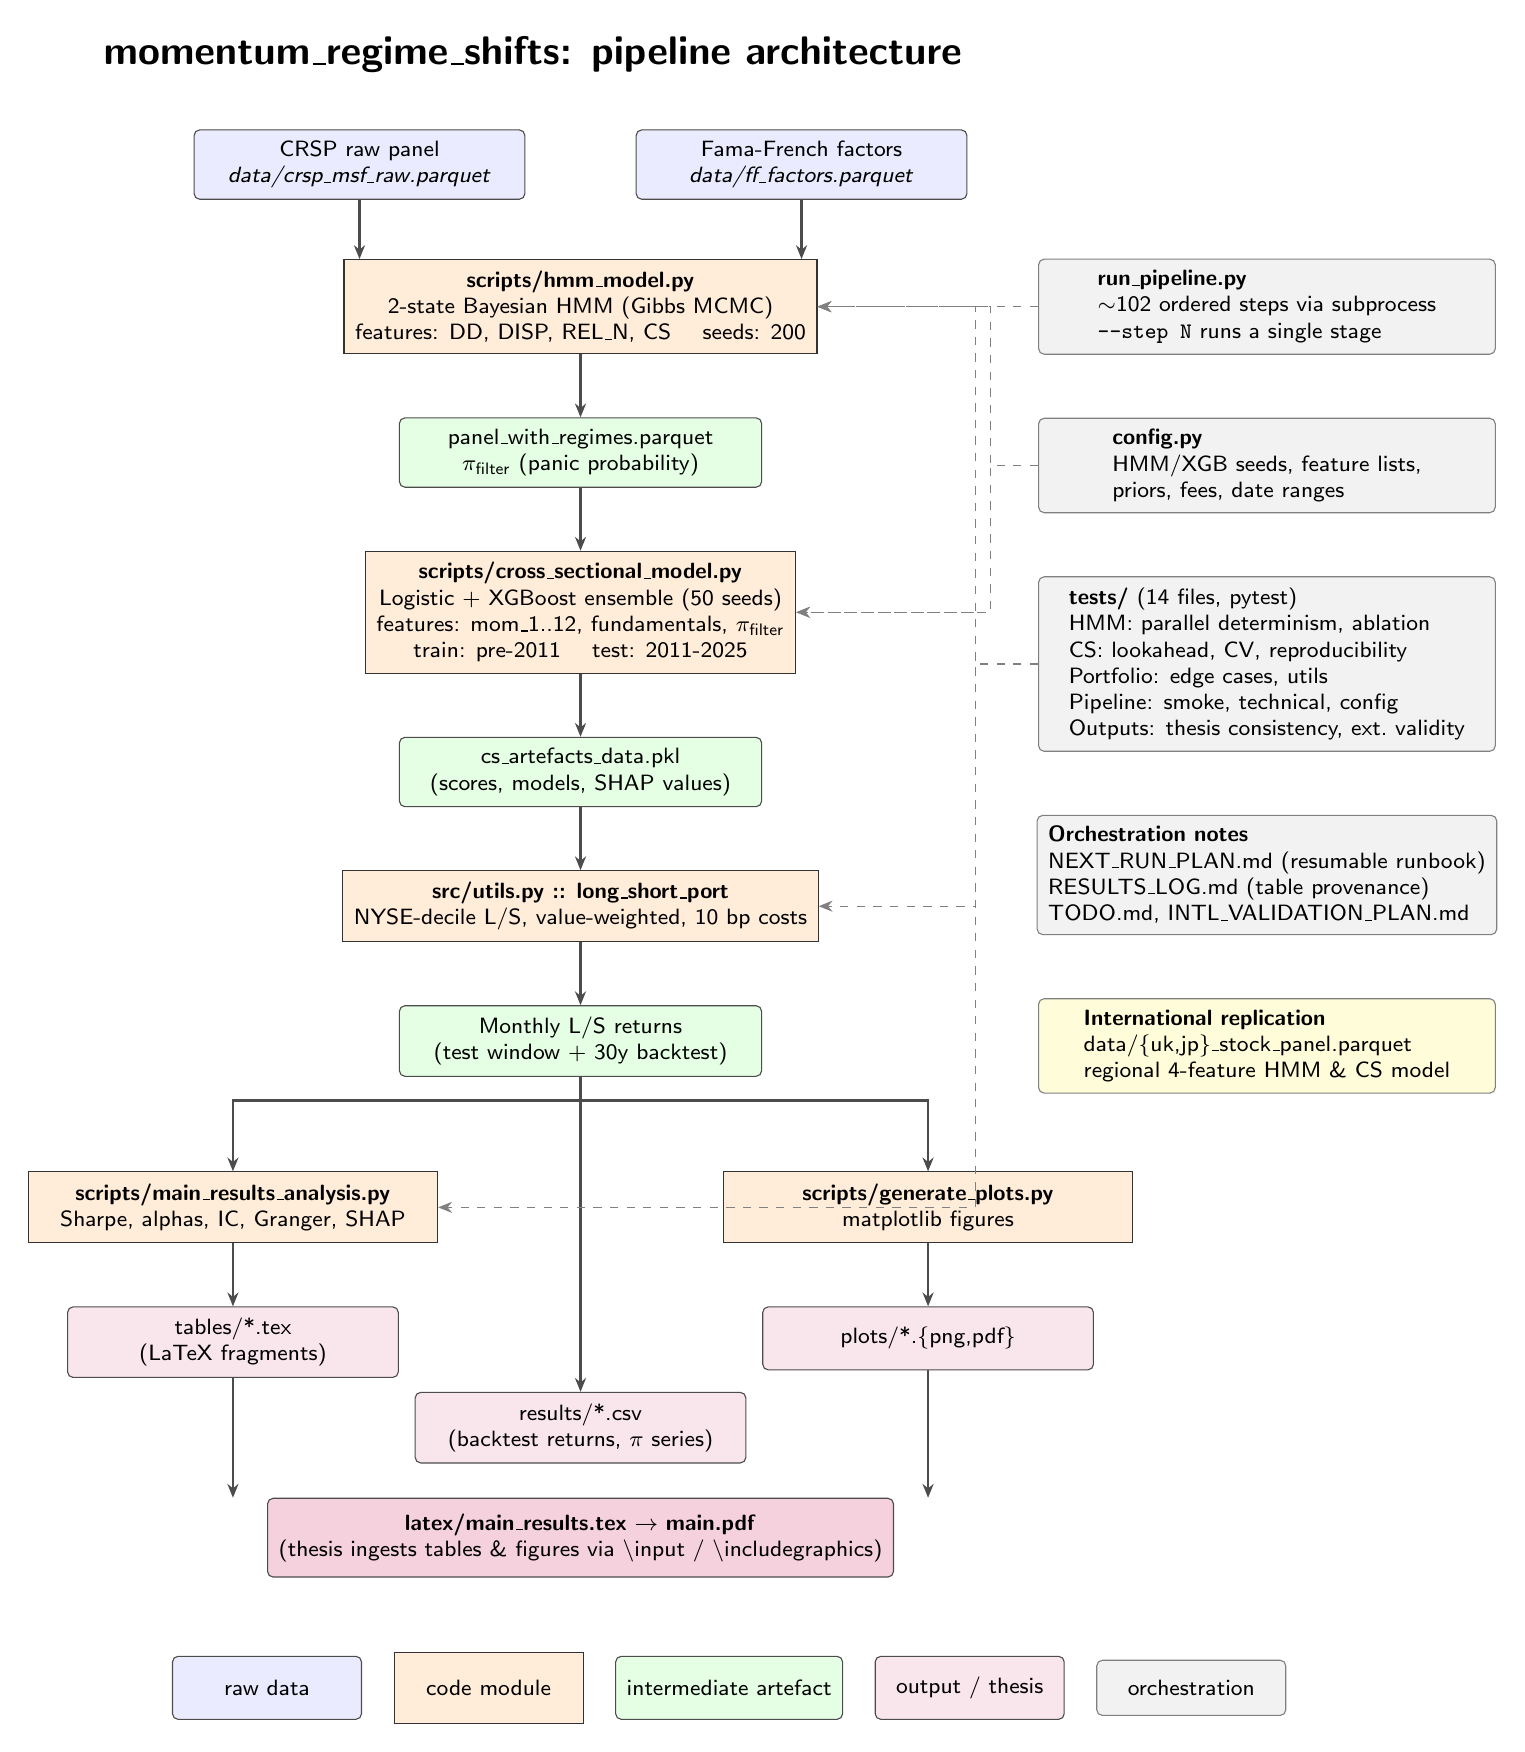
\begin{tikzpicture}[
    font=\footnotesize,
    >={Stealth[length=5pt,width=4pt]},
    node distance=8mm and 10mm,
    data/.style    ={rectangle, rounded corners=2pt, draw=black!70, fill=blue!8,   minimum height=8mm, minimum width=42mm, align=center, inner sep=4pt},
    code/.style    ={rectangle,                  draw=black!80, fill=orange!15, minimum height=9mm, minimum width=52mm, align=center, inner sep=4pt},
    artefact/.style={rectangle, rounded corners=2pt, draw=black!70, fill=green!10,  minimum height=8mm, minimum width=46mm, align=center, inner sep=4pt},
    output/.style  ={rectangle, rounded corners=2pt, draw=black!70, fill=purple!10, minimum height=8mm, minimum width=42mm, align=center, inner sep=4pt},
    side/.style    ={rectangle, rounded corners=2pt, draw=black!50, fill=gray!10,   minimum height=7mm, minimum width=46mm, align=left,   inner sep=4pt},
    grouplabel/.style={font=\small\bfseries, text=black!70},
    arrow/.style={->, thick, draw=black!70},
    sidearrow/.style={->, dashed, draw=black!50},
]

%==================== MAIN PIPELINE COLUMN ====================

\node[data] (crsp)   {CRSP raw panel\\\textit{data/crsp\_msf\_raw.parquet}};
\node[data, right=14mm of crsp] (ff) {Fama-French factors\\\textit{data/ff\_factors.parquet}};

% HMM stage
\node[code, below=12mm of $(crsp)!0.5!(ff)$] (hmm) {\textbf{scripts/hmm\_model.py}\\2-state Bayesian HMM (Gibbs MCMC)\\features: DD, DISP, REL\_N, CS \quad seeds: 200};

\node[artefact, below=of hmm] (panel) {panel\_with\_regimes.parquet\\$\pi_{\text{filter}}$ (panic probability)};

% Cross-sectional stage
\node[code, below=of panel] (cs) {\textbf{scripts/cross\_sectional\_model.py}\\Logistic + XGBoost ensemble (50 seeds)\\features: mom\_1..12, fundamentals, $\pi_{\text{filter}}$\\train: pre-2011 \quad test: 2011-2025};

\node[artefact, below=of cs] (artef) {cs\_artefacts\_data.pkl\\(scores, models, SHAP values)};

% Portfolio stage
\node[code, below=of artef] (port) {\textbf{src/utils.py :: long\_short\_port}\\NYSE-decile L/S, value-weighted, 10 bp costs};

\node[artefact, below=of port] (rets) {Monthly L/S returns\\(test window + 30y backtest)};

%==================== AGGREGATION FAN-OUT ====================

\node[code, below left=12mm and -5mm of rets] (mainres) {\textbf{scripts/main\_results\_analysis.py}\\Sharpe, alphas, IC, Granger, SHAP};
\node[code, below right=12mm and -5mm of rets] (plots)   {\textbf{scripts/generate\_plots.py}\\matplotlib figures};

\node[output, below=of mainres] (tables) {tables/*.tex\\(LaTeX fragments)};
\node[output, below=of plots]   (figs)   {plots/*.\{png,pdf\}};
\node[output, below=18mm of rets, yshift=-22mm] (csvs) {results/*.csv\\(backtest returns, $\pi$ series)};

% Thesis
\node[output, below=20mm of $(tables)!0.5!(figs)$, fill=purple!18, minimum width=70mm, minimum height=10mm] (thesis)
  {\textbf{latex/main\_results.tex} $\rightarrow$ \textbf{main.pdf}\\(thesis ingests tables \& figures via \textbackslash input / \textbackslash includegraphics)};

%==================== ARROWS (main flow) ====================

\draw[arrow] (crsp.south) -- (hmm.north -| crsp.south);
\draw[arrow] (ff.south)   -- (hmm.north -| ff.south);
\draw[arrow] (hmm)   -- (panel);
\draw[arrow] (panel) -- (cs);
\draw[arrow] (cs)    -- (artef);
\draw[arrow] (artef) -- (port);
\draw[arrow] (port)  -- (rets);

\draw[arrow] (rets.south) -- ++(0,-3mm) -| (mainres.north);
\draw[arrow] (rets.south) -- ++(0,-3mm) -| (plots.north);
\draw[arrow] (rets.south) -- ++(0,-3mm) -| (csvs.north);

\draw[arrow] (mainres) -- (tables);
\draw[arrow] (plots)   -- (figs);

\draw[arrow] (tables.south) -- (thesis.north -| tables.south);
\draw[arrow] (figs.south)   -- (thesis.north -| figs.south);

%==================== SIDE PANEL: ORCHESTRATION ====================

\node[side, right=28mm of hmm, anchor=west, minimum width=58mm] (run)
  {\textbf{run\_pipeline.py}\\$\sim$102 ordered steps via subprocess\\\texttt{--step N} runs a single stage};

\node[side, below=of run, minimum width=58mm] (cfg)
  {\textbf{config.py}\\HMM/XGB seeds, feature lists,\\priors, fees, date ranges};

\node[side, below=of cfg, minimum width=58mm] (tests)
  {\textbf{tests/} (14 files, pytest)\\HMM: parallel determinism, ablation\\CS: lookahead, CV, reproducibility\\Portfolio: edge cases, utils\\Pipeline: smoke, technical, config\\Outputs: thesis consistency, ext.\ validity};

\node[side, below=of tests, minimum width=58mm] (notes)
  {\textbf{Orchestration notes}\\NEXT\_RUN\_PLAN.md (resumable runbook)\\RESULTS\_LOG.md (table provenance)\\TODO.md, INTL\_VALIDATION\_PLAN.md};

\node[side, below=of notes, minimum width=58mm, fill=yellow!15] (intl)
  {\textbf{International replication}\\data/\{uk,jp\}\_stock\_panel.parquet\\regional 4-feature HMM \& CS model};

% dashed influence arrows from orchestration to pipeline
\draw[sidearrow] (run.west)   -- ++(-4mm,0) |- (hmm.east);
\draw[sidearrow] (cfg.west)   -- ++(-6mm,0) |- (cs.east);
\draw[sidearrow] (cfg.west)   -- ++(-6mm,0) |- (hmm.east);
\draw[sidearrow] (tests.west) -- ++(-8mm,0) |- (hmm.east);
\draw[sidearrow] (tests.west) -- ++(-8mm,0) |- (cs.east);
\draw[sidearrow] (tests.west) -- ++(-8mm,0) |- (port.east);
\draw[sidearrow] (tests.west) -- ++(-8mm,0) |- (mainres.east);

%==================== LEGEND ====================

\begin{scope}[shift={($(thesis.south west)+(0,-14mm)$)}]
  \node[data,     minimum width=24mm] (l1) at (0,0) {raw data};
  \node[code,     minimum width=24mm, right=4mm of l1] (l2) {code module};
  \node[artefact, minimum width=24mm, right=4mm of l2] (l3) {intermediate artefact};
  \node[output,   minimum width=24mm, right=4mm of l3] (l4) {output / thesis};
  \node[side,     minimum width=24mm, right=4mm of l4] (l5) {orchestration};
\end{scope}

%==================== TITLE ====================

\node[font=\Large\bfseries, above=6mm of crsp, xshift=22mm] {momentum\_regime\_shifts: pipeline architecture};

\end{tikzpicture}
\end{document}
